% 
% chapter3.tex
% ThesisISEL
% 
% Created by Serge Lage on 2019/07/30.
%
% ================
% = Data =
% ================
\chapter{Data Analysis}
\label{cha:data}


\section{Descriptive Data Analysis} % (fold)
\label{sub:data_analysis}



The data used as input to the models is VMS Records data. Among these data, those that best distinguish between different types of fishing activity are speed and location.\\
About the locations, certain fishing types only occur in certain depth. So the locations can help in these cases. \\
To meet the objectives, we need to understand the velocity patterns.
By studying and analyzing the velocity data, it was possible to verify the existence of two velocity distributions.

\begin{figure}[h]
\centering
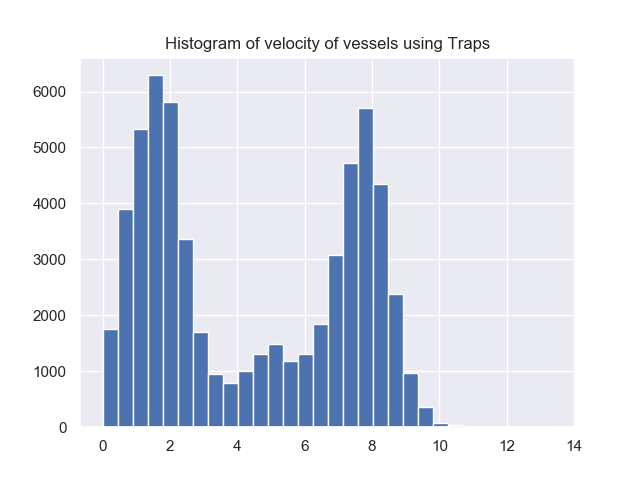
\includegraphics[width=0.8\linewidth]{Chapters/img/h_armadilhas.png}
\caption{Histogram of velocity of traps license.}
\label{fig:h_armadilhas}
\end{figure}

%\begin{figure}[h]
% \centering
% 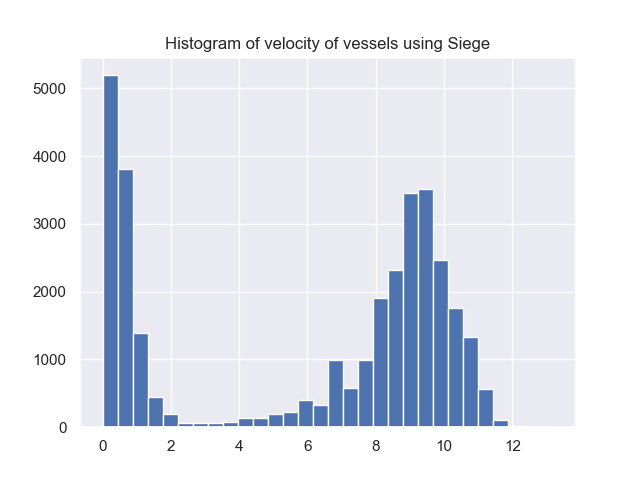
\includegraphics[width=0.8\linewidth]{Chapters/img/h_cerco.png}
% \caption{Histogram of velocity of siege license.}
% \label{fig:h_cerco}
%\end{figure}

\begin{figure}[h]
\centering
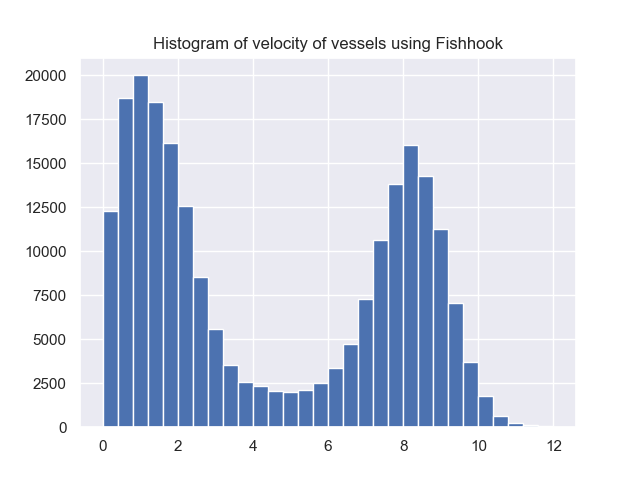
\includegraphics[width=0.8\linewidth]{Chapters/img/h_linha.png}
\caption{Histogram of velocity of fishhook license.}
\label{fig:h_linha}
\end{figure}

In Figure \ref{fig:h_armadilhas} it is possible to distinguish two different speed distributions, the lower speeds correspond to fishing activities, and the higher speeds represent the movements of the vessel from the port to the fishing grounds and back to the port \cite{MappingFishing}.





Knowing this, we can notice that different types of fishing have different fishing speeds, as we can see the differences between the histogram in Figure \ref{fig:h_armadilhas} containing data on fishing vessels using traps and Figure \ref{fig:h_linha} concerning fishing vessels using fishhook.





It is essential to separate the inputs representing fishing speeds from the others in the data as the input to the models used in Chapter 5 it is necessary to have the data filtered out only with the fishing activity data. This is because we will only use the fishing speed to study and create the methodology's necessary to achieve the proposed goals.

Data from operations different from fisheries should be discarded as they do not discriminate against different types of fishing. For example, speed 0 nautical miles is not interesting regardless of their type of fishing, once all vessels stop in the fishing port.


% section data_analysis (end)

% chapter data (end)




